\documentclass[10pt,a4paper]{article}
\usepackage[utf8]{inputenc}
\usepackage{amsmath}
\usepackage{amsfonts}
\usepackage{amssymb}
\usepackage{graphicx}
\author{Pranav Satheesh|PH17B008}
\title{PH5270 Numerical Methods and Programming Lab Assignment}
\begin{document}

\maketitle

\section*{Damped driven pendulum}
For this assignment we are looking at the case of a damped pendulum subject to an external driving force. First off, we should write down the equation of motion for this system. This is fairly straight forward but let's begin with identifying and setting some values of parameters in this problem.

\begin{itemize}
\item Mass of the body $m=1$
\item Length of the string $l=1$
\item $\beta = \sqrt{\frac{g}{l}}$ and also setting $g=1$
\item Damping force parameter $k$. The damping force is $-m k \omega$, where $\omega = \dot{\theta}$
\item The driving force is given by $m A cos(\Omega t)$, where A is the Amplitude of the driving force and $\Omega$ is the frequency. 
\end{itemize}

The equation of motion can be written as,

\begin{align}
\dot{\theta}&=\omega\\
\dot{\omega}&= -\beta^2 sin \theta - k \omega + A cos(\Omega t) 
\end{align}

\section*{Step-1}

\subsection*{(i) Euler predictor-corrector method}

By averaging Euler and backward Euler methods we can achieve higher-order accuracy.

\emph{The Predictor step}
\begin{align}
\tilde{\theta_{k + 1}}&= \theta_k + h \omega_k(t_k)\\
\tilde{\omega_{k + 1}}&= \omega_k + h f(t_k,\theta_k,\omega_k)
\end{align}

\emph{The corrector step}
\begin{align}
\theta_{k + 1}&= \theta_k + \frac{h}{2}(\omega_k(t_k) \tilde{\omega_{k + 1}})\\
\omega_{k + 1}&= \omega_k + h (f(t_k,\theta_k,\omega_k) + f(t_{k+1}, \tilde{theta_{k+1}}, \tilde{\omega_{k+1}})
\end{align}

Where $f(\theta_k,\omega_k,t_k) = -\beta^2 sin \theta - k \omega + A cos(\Omega t) $

To determine the accuracy of this algorithm, we apply it to a scalar ODE $ x^{,} = \lambda x$, obtaining

$$ x_k = \left(\frac{1 + h \frac{\lambda}{2}}{1 - h \frac{\lambda}{2}} \right)^{k} x_0 $$

The growth factor when epanded out gives,

$$ \frac{1 + h \frac{\lambda}{2}}{1 - h \frac{\lambda}{2}} = 1 + h \lambda + \frac{(h \lambda)^2}{2} + \frac{(h \lambda)^3}{4} + \dots $$

This agrees with expression of $e^{h \lambda}$ through terms of order $h^2$, so this algorithm is \textbf{second-order accurate}.

\subsection*{(ii)Taylor series methods}

This algorithm uses Taylor series expansion to solve the ODE.

From the Taylor series expansion of x(t+h), we truncate till second order for a \emph{second-order} method.

$$ x_{k+1} = x_k + h x^{'}_k + \frac{h^{2}}{2} x^{''}_k $$

The higher derivatives of x can be obtained by differentiating $x^{'} = f(t,x)$ using chain rule.

$$ x^{''} = f_t (t,x) + f_x (t,x) f(t,x) $$

Now applying this algorithm to the equations of motion in this problem we get:

\begin{align}
\theta_{k+1}&=\theta_k + h \omega_k + \frac{h^2}{2} \theta^{''}_k\\
\theta^{''}_k&= f(\theta_k,\omega_k,t)\\
\end{align}

\begin{align}
\omega_{k+1}&=\omega_k + h f(\theta_k,\omega_k,t) + \frac{h^2}{2} \omega^{''}_k\\
\omega^{''}_k&= \frac{f(\theta,\omega,t)}{dt}\\
&= -\beta^2 \omega \ cos \theta - A \Omega \ sin(\Omega t) - k f(\theta_k,\omega_k,t)
\end{align}
 
This method is also \textbf{second-order} accurate.

\subsection*{(iii)Second-order Runge-Kutta methods}

Runge-Kutta methods are a class of methods which judiciously uses the information on the 'slope' at more than one point to extrapolate the solution to the future time step.

For the ODE $\frac{d y}{d t} = f(t, y(t))$
\begin{align*}
k1&= h f(t,y(t))\\
k2&= h f(t + \frac{h}{2},y(t) + \frac{k1}{2})\\
y(t+h)&= y(t) + k_2
\end{align*}

This is also \textbf{second-order} accurate as it is evident from the expansion of $y(t+h):$

$$ y_{n+1} = y_n + h f(y_n,t_n) + \frac{1}{2} h^2 (\frac{\partial f}{\partial t} + f \frac{\partial f}{\partial y})(y_n,t_n) + \mathcal{O}(h^3)$$


\subsection*{(iv)Fourth-order Runge-Kutta methods}

We can increase the efficiency of the Runge-Kutta method by calculating more slopes. $k_1$ at the beginning of the interval. $k_2$ is the slope at the midpoint of the interval, using y and $k_1$. $k_3$ is the slope at the midpoint, but now using y and $k_2$.$k_{4}$ is the slope at the end of the interval, using y and $k_{3}$.In averaging the four slopes, greater weight is given to the slopes at the midpoint.\\



For the ODE, $$\frac{d y}{d t} = f(t, y(t))$$

\begin{align*}
k1&=h f(t_n,y_n)\\
k2&=h f(t_n + \frac{h}{2},y_n + \frac{k1}{2})\\
k3&=h f(t_n + \frac{h}{2},y_n +  \frac{k2}{2})\\
k4&= h f(t_n + h,y_n + h k_3)\\
\end{align*}

\begin{align*}
y_{n+1}&= y_n + \frac{1}{6} h (k_1 + 2 k_2 + 2 k_3 + k_4)\\
t_{n+1}&= t_n + h
\end{align*}

This Method is \textbf{fourth-order accurate}.

\section*{Step-2}

The files Odefunctions.h, Odefunctions.cpp and main.cpp contains code for solving the ODE for various cases and user's choice of algorithm. User can give values of the parameter ($A,k,\Omega$) , step size $dt$ and the total number of steps $N$. The user can input the file name as well. The file name begins with the user's choice of algorithm. The various data files thus obtained are available in this directory. The plots are done using GNUPLOT. I have used six GNUPLOT scripts for my individual plots.

\subsection*{Inference}

This section discusses my plots and the various conclusions that can be draen from it.

\subsubsection*{Comparing the four algorithms used}
 

\begin{figure}[h]
\centering
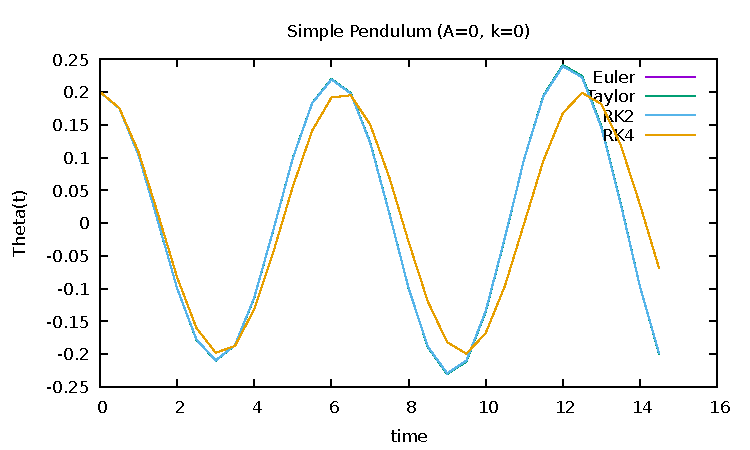
\includegraphics[scale=0.9]{method_comparison.pdf}
\caption{Simple pendulum case for the 4 different methods}
\label{Fig1}
\end{figure}

In this plot, I'm considering the simple pendulum case ($A=0,k=0$) for all the four methods considering a fixed time step (0.5) and number of points (30). The plot [\ref{Fig1}] clearly shows a match for Euler,Taylor and Runge-Kutta order 2 (RK2) methods. This is because they all are \textbf{2nd order} methods. Whereas, the \textbf{4th order} accurate \emph{Runge-Kutta} (RK4) is different from the rest. Clearly, RK4 is the best and the most accurate method among the four algorithms discussed here.\\

\newpage
\subsubsection*{Comparing the effect of time-step}


\begin{figure}[h]
\centering
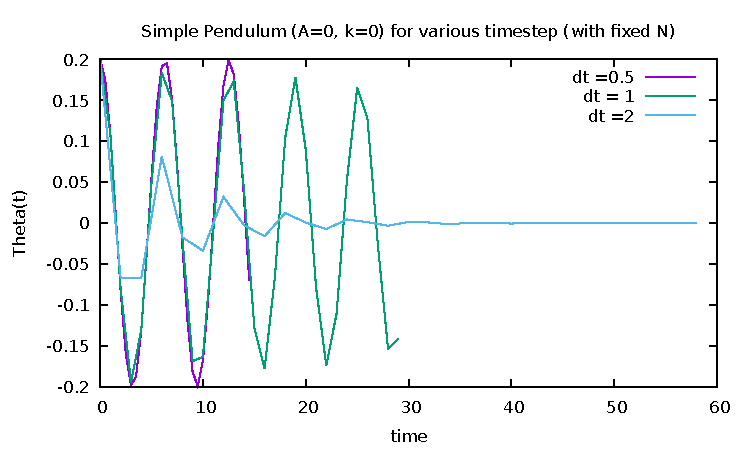
\includegraphics[scale=0.9]{timestep_comparison.pdf}
\caption{Simple pendulum case for different time steps}
\label{Fig2}
\end{figure}

Here I'm plotting [\ref{Fig2}] the simple pendulum case for three different time steps $dt = 0.5,1,2$ for fixed number of points (30). We find that a smaller time step (0.5) reduces the error compared to a time step like 2.

\subsubsection*{Various physical situations}

\begin{figure}[h]
\centering
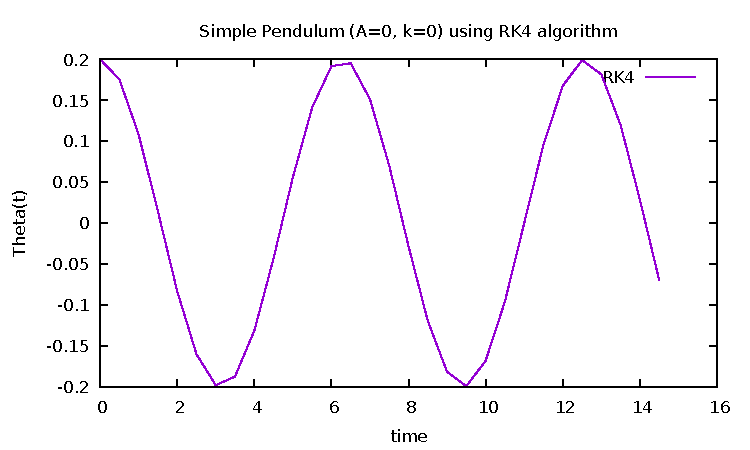
\includegraphics[scale=0.9]{Simple_Pendulum.pdf}
\caption{Simple pendulum case using RK4}
\label{Fig3}
\end{figure}

The most straightforwad case is the simple pendulum which is basically a sinusoid [\ref{Fig3}].

\begin{figure}[h]
\centering
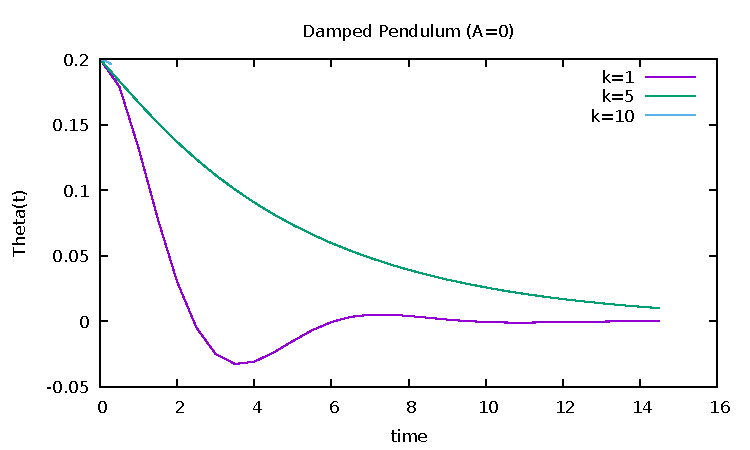
\includegraphics[scale=0.9]{damped_pendulum.pdf}
\caption{Damped pendulum case using RK4}
\label{Fig4}
\end{figure}

The damped pendulum plot [\ref{Fig4}] shows that when you increaseing the damping parameter (k) the pendulum dies of quickly. As evident from the case of k=5. k=10 is even faster but it is not clearly visible in [\ref{Fig4}]

Here's a version of the plot featuring only k=10. Look how quickly the motion dampends to zero.

\begin{figure}[h]
\centering
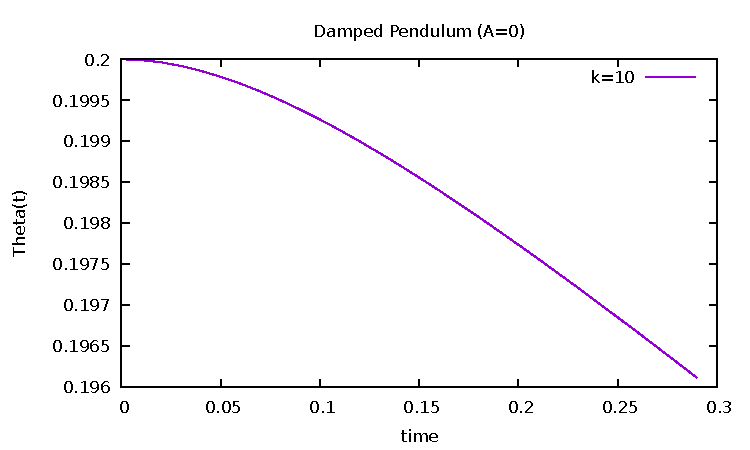
\includegraphics[scale=0.9]{damped_pendulum3.pdf}
\caption{Damped pendulum case using RK4 for k=10}
\label{Fig5}
\end{figure}

\newpage

\begin{figure}[h]
\centering
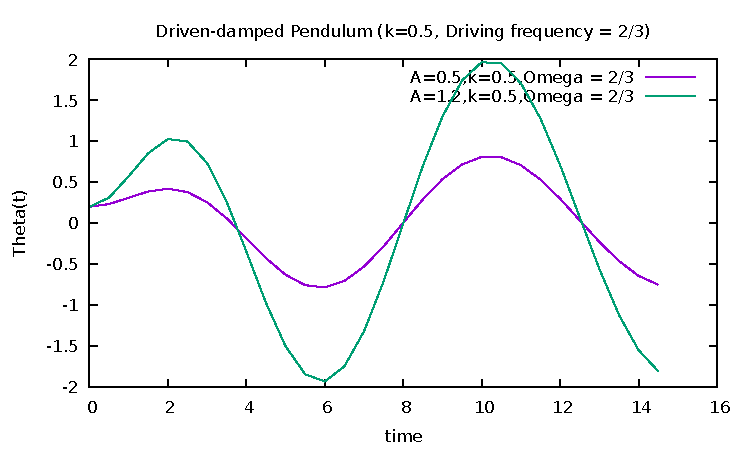
\includegraphics[scale=0.9]{driven_pendulum.pdf}
\caption{Damped-Driven pendulum case using RK4}
\label{Fig6}
\end{figure}

The final case is the driven pendulum [\ref{Fig6}]. Evidently the driving force forces it away from damping and it achieves the amplitude of the driving force given at some point. When the frequency of the pendulum reaches the driving force frequency, the pendulum is in \emph{resonance}.

\end{document}
